%===============================================================================
% LaTeX sjabloon voor de graduaatsproef Programmeren aan HOGENT
% Meer info op https://github.com/HoGentPRG/latex-hogent-report
%===============================================================================

\documentclass[english,dit,thesis]{hogentreport}

% TODO:
% - If necessary, replace the option `dit`' with your own department!
%   Valid entries are dbo, dbt, dgz, dit, dlo, dog, dsa, soa
% - If you write your thesis in English (remark: only possible after getting
%   explicit approval!), remove the option "dutch," or replace with "english".

% \usepackage{lipsum} % For blind text, can be removed after adding actual content

%% Pictures to include in the text can be put in the graphics/ folder
\graphicspath{{../graphics/}}

%% For source code highlighting, requires pygments to be installed
%% Compile with the -shell-escape flag!
%% \usepackage[chapter]{minted}
%% If you compile with the make_thesis.{bat,sh} script, use the following
%% import instead:
\usepackage[chapter,outputdir=../output]{minted}
\usemintedstyle{solarized-light}

%% Formatting for minted environments.
\setminted{%
    autogobble,
    frame=lines,
    breaklines,
    linenos,
    tabsize=4
}

%% Ensure the list of listings is in the table of contents
\renewcommand\listoflistingscaption{%
    \IfLanguageName{dutch}{Lijst van codefragmenten}{List of listings}
}
\renewcommand\listingscaption{%
    \IfLanguageName{dutch}{Codefragment}{Listing}
}
\renewcommand*\listoflistings{%
    \cleardoublepage\phantomsection\addcontentsline{toc}{chapter}{\listoflistingscaption}%
    \listof{listing}{\listoflistingscaption}%
}

% Other packages not already included can be imported here

%%---------- Document metadata -------------------------------------------------
% TODO: Replace this with your own information
\author{Rafal Kowalski}
\supervisor{Luc Vervoort}
\cosupervisor{Wim Goedertier}
\title[\IfLanguageName{dutch}{Voordelen en uitdagingen van één enkele codebron}{Advantages and challenges of a single source codebase}]{
    \IfLanguageName{dutch}{Cross-platform applicatie met Vue, \newline Quasar en NestJS}{Cross platform application with Vue, \newline Quasar and NestJS}
}
\academicyear{\advance\year by -1 \the\year--\advance\year by 1 \the\year}
\examperiod{1}
\degreesought{\IfLanguageName{dutch}{Graduaat in het Programmeren}{Associate of applied computer science}}
\partialthesis{false} %% To display 'in partial fulfilment'
%\institution{Internshipcompany BVBA.}

%% Add global exceptions to the hyphenation here
\hyphenation{back-slash}

%% The bibliography (style and settings are  found in hogentthesis.cls)
% \addbibresource{./gradproef.bib}          %% Bibliography file
% \addbibresource{../voorstel/voorstel.bib} %% Bibliography research proposal
\addbibresource{../bibs/proef.bib}          %% Combined Bibliography file
\defbibheading{bibempty}{}

%% Prevent empty pages for right-handed chapter starts in twoside mode
\renewcommand{\cleardoublepage}{\clearpage}

\renewcommand{\arraystretch}{1.2}

%% Content starts here.
\begin{document}

%---------- Front matter -------------------------------------------------------

\frontmatter

\hypersetup{pageanchor=false} %% Disable page numbering references
%% Render a Dutch outer title page if the main language is English
\IfLanguageName{english}{%
    %% If necessary, information can be changed here
    \degreesought{Graduaat in het Programmeren}%
    \begin{otherlanguage}{dutch}%
       \maketitle%
    \end{otherlanguage}%
}{}

%% Generates title page content
\maketitle
\hypersetup{pageanchor=true}

%%=============================================================================
%% Voorwoord
%%=============================================================================

\chapter*{\IfLanguageName{dutch}{Woord vooraf}{Preface}}%
\label{ch:voorwoord}

TODO:
Het voorwoord is het enige deel van de graduaatsproef waar je vanuit je
eigen standpunt (``ik-vorm'') mag schrijven. Je kan hier bv. motiveren
waarom jij het onderwerp wil bespreken.
Vergeet ook niet te bedanken wie je geholpen/gesteund/... heeft

%%=============================================================================
%% Samenvatting
%%=============================================================================

% TODO: De "abstract" of samenvatting is een kernachtige (~ 1 blz. voor een
% thesis) synthese van het document.
%
% Een goede abstract biedt een kernachtig antwoord op volgende vragen:
%
% 1. Waarover gaat de graduaatsproef?
% 2. Waarom heb je er over geschreven?
% 3. Hoe heb je het onderzoek uitgevoerd?
% 4. Wat waren de resultaten? Wat blijkt uit je onderzoek?
% 5. Wat betekenen je resultaten? Wat is de relevantie voor het werkveld?
%
% Daarom bestaat een abstract uit volgende componenten:
%
% - inleiding + kaderen thema
% - probleemstelling
% - (centrale) onderzoeksvraag
% - onderzoeksdoelstelling
% - methodologie
% - resultaten (beperk tot de belangrijkste, relevant voor de onderzoeksvraag)
% - conclusies, aanbevelingen, beperkingen
%
% LET OP! Een samenvatting is GEEN voorwoord!

%%---------- Nederlandse samenvatting -----------------------------------------
%
% TODO: Als je je graduaatsproef in het Engels schrijft, moet je eerst een
% Nederlandse samenvatting invoegen. Haal daarvoor onderstaande code uit
% commentaar.
% Wie zijn/haar graduaatsproef in het Nederlands schrijft, kan dit negeren, de inhoud
% wordt niet in het document ingevoegd.

\IfLanguageName{english}{%
\selectlanguage{dutch}
\chapter*{Samenvatting}
\lipsum[1-4]
\selectlanguage{english}
}{}

%%---------- Samenvatting -----------------------------------------------------
% De samenvatting in de hoofdtaal van het document

\chapter*{\IfLanguageName{dutch}{Samenvatting}{Abstract}}

\lipsum[1-4]


%---------- Inhoud, lijst figuren, ... -----------------------------------------

\tableofcontents

% In a list of figures, the complete caption will be included. To prevent this,
% ALWAYS add a short description in the caption!
%
%  \caption[short description]{elaborate description}
%
% If you do, only the short description will be used in the list of figures

\listoffigures

% If you included tables and/or source code listings, uncomment the appropriate
% lines.
\listoftables

\listoflistings

% Als je een lijst van afkortingen of termen wil toevoegen, dan hoort die
% hier thuis. Gebruik bijvoorbeeld de ``glossaries'' package.
% https://www.overleaf.com/learn/latex/Glossaries

%---------- Kern ---------------------------------------------------------------

\mainmatter{}

% De eerste hoofdstukken van een graduaatsproef zijn meestal een inleiding op
% het onderwerp, literatuurstudie en verantwoording methodologie.
% Aarzel niet om een meer beschrijvende titel aan deze hoofdstukken te geven of
% om bijvoorbeeld de inleiding en/of stand van zaken over meerdere hoofdstukken
% te verspreiden!

%%=============================================================================
%% Inleiding
%%=============================================================================

\chapter{\IfLanguageName{dutch}{Inleiding}{Introduction}}%
\label{ch:inleiding}

% De inleiding moet de lezer net genoeg informatie verschaffen om het onderwerp te begrijpen en in te zien waarom de onderzoeksvraag de moeite waard is om te onderzoeken. 
% In de inleiding ga je literatuurverwijzingen beperken, zodat de tekst vlot leesbaar blijft. 
% Je kan de inleiding verder onderverdelen in secties als dit de tekst verduidelijkt. Zaken die aan bod kunnen komen in de inleiding:

% \begin{itemize}
%   \item context, achtergrond
%   \item afbakenen van het onderwerp
%   \item verantwoording van het onderwerp, methodologie
%   \item probleemstelling
%   \item onderzoeksdoelstelling
%   \item onderzoeksvraag
%   \item \ldots
% \end{itemize}

\section{\IfLanguageName{dutch}{Probleemstelling}{Problem Statement}}%
\label{sec:probleemstelling}

% Uit je probleemstelling moet duidelijk zijn dat je onderzoek een meerwaarde heeft voor een concrete doelgroep. 
% De doelgroep moet goed gedefinieerd en afgelijnd zijn. Doelgroepen als ``bedrijven,'' ``KMO's'', systeembeheerders, enz.~zijn nog te vaag. 
% Als je een lijstje kan maken van de personen/organisaties die een meerwaarde zullen vinden in deze bachelorproef (dit is eigenlijk je steekproefkader), dan is dat een indicatie dat de doelgroep goed gedefinieerd is. 
% Dit kan een enkel bedrijf zijn of zelfs één persoon (je co-promotor/opdrachtgever).

\section{\IfLanguageName{dutch}{Onderzoeksvraag}{Research question}}%
\label{sec:onderzoeksvraag}

% Wees zo concreet mogelijk bij het formuleren van je onderzoeksvraag. 
% Een onderzoeksvraag is trouwens iets waar nog niemand op dit moment een antwoord heeft (voor zover je kan nagaan). 
% Het opzoeken van bestaande informatie (bv. ``welke tools bestaan er voor deze toepassing?'') is dus geen onderzoeksvraag. 
% Je kan de onderzoeksvraag verder specifiëren in deelvragen. Bv.~als je onderzoek gaat over performantiemetingen, dan 

\section{\IfLanguageName{dutch}{Onderzoeksdoelstelling}{Research objective}}%
\label{sec:onderzoeksdoelstelling}

% Wat is het beoogde resultaat van je graduaatsproef? 
% Wat zijn de criteria voor succes? Beschrijf die zo concreet mogelijk. 
% Gaat het bv.\ om een proof-of-concept, een prototype, een verslag met aanbevelingen, een vergelijkende studie, enz.

\section{\IfLanguageName{dutch}{Opzet van deze graduaatsproef}{Structure of this associate thesis}}%
\label{sec:opzet-graduaatsproef}

% Het is gebruikelijk aan het einde van de inleiding een overzicht te
% geven van de opbouw van de rest van de tekst. Deze sectie bevat al een aanzet
% die je kan aanvullen/aanpassen in functie van je eigen tekst.\newline

% De rest van deze graduaatsproef is als volgt opgebouwd:

% In Hoofdstuk~\ref{ch:stand-van-zaken} wordt een overzicht gegeven van de stand van zaken binnen het onderzoeksdomein, op basis van een literatuurstudie.\newline

% In Hoofdstuk~\ref{ch:methodologie} wordt de methodologie toegelicht en worden de gebruikte onderzoekstechnieken besproken om een antwoord te kunnen formuleren op de onderzoeksvragen.

% TODO: Vul hier aan voor je eigen hoofstukken, één of twee zinnen per hoofdstuk

% In Hoofdstuk~\ref{ch:conclusie}, tenslotte, wordt de conclusie gegeven en een antwoord geformuleerd op de onderzoeksvragen. Daarbij wordt ook een aanzet gegeven voor toekomstig onderzoek binnen dit domein.
\chapter{\IfLanguageName{dutch}{Stand van zaken}{State of the art}}%
\label{ch:stand-van-zaken}

% Tip: Begin elk hoofdstuk met een paragraaf inleiding die beschrijft hoe
% dit hoofdstuk past binnen het geheel van de graduaatsproef. Geef in het
% bijzonder aan wat de link is met het vorige en volgende hoofdstuk.

% Pas na deze inleidende paragraaf komt de eerste sectiehoofding.

Dit hoofdstuk bevat je literatuurstudie. De inhoud gaat verder op de inleiding, maar zal het onderwerp van de graduaatsproef *diepgaand* uitspitten. De bedoeling is dat de lezer na lezing van dit hoofdstuk helemaal op de hoogte is van de huidige stand van zaken (state-of-the-art) in het onderzoeksdomein. Iemand die niet vertrouwd is met het onderwerp, weet nu voldoende om de rest van het verhaal te kunnen volgen, zonder dat die er nog andere informatie moet over opzoeken \autocite{Pollefliet2011}.

Je verwijst bij elke bewering die je doet, vakterm die je introduceert, enz.\ naar je bronnen. In \LaTeX{} kan dat met het commando \texttt{$\backslash${textcite\{\}}} of \texttt{$\backslash${autocite\{\}}}. Als argument van het commando geef je de ``sleutel'' van een ``record'' in een bibliografische databank in het Bib\LaTeX{}-formaat (een tekstbestand). Als je expliciet naar de auteur verwijst in de zin (narratieve referentie), gebruik je \texttt{$\backslash${}textcite\{\}}. Soms is de auteursnaam niet expliciet een onderdeel van de zin, dan gebruik je \texttt{$\backslash${}autocite\{\}} (referentie tussen haakjes). Dit gebruik je bv.~bij een citaat, of om in het bijschrift van een overgenomen afbeelding, broncode, tabel, enz. te verwijzen naar de bron. In de volgende paragraaf een voorbeeld van elk.

\textcite{Knuth1998} schreef een van de standaardwerken over sorteer- en zoekalgoritmen. Experten zijn het erover eens dat cloud computing een interessante opportuniteit vormen, zowel voor gebruikers als voor dienstverleners op vlak van informatietechnologie~\autocite{Creeger2009}.

Let er ook op: het \texttt{cite}-commando voor de punt, dus binnen de zin. Je verwijst meteen naar een bron in de eerste zin die erop gebaseerd is, dus niet pas op het einde van een paragraaf.

\begin{figure}
  \centering
  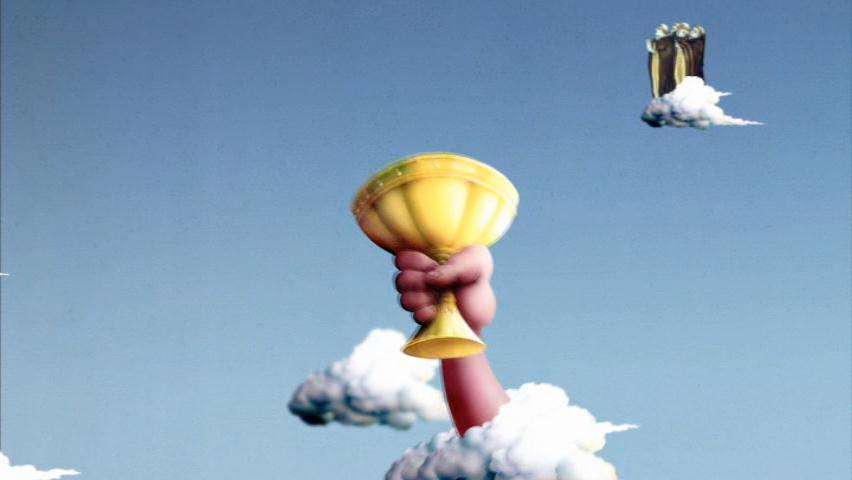
\includegraphics[width=0.8\textwidth]{grail.jpg}
  \caption[Voorbeeld figuur.]{\label{fig:grail}Voorbeeld van invoegen van een figuur. Zorg altijd voor een uitgebreid bijschrift dat de figuur volledig beschrijft zonder in de tekst te moeten gaan zoeken. Vergeet ook je bronvermelding niet!}
\end{figure}

\begin{listing}
  \begin{minted}{python}
    import pandas as pd
    import seaborn as sns

    penguins = sns.load_dataset('penguins')
    sns.relplot(data=penguins, x="flipper_length_mm", y="bill_length_mm", hue="species")
  \end{minted}
  \caption[Voorbeeld codefragment]{Voorbeeld van het invoegen van een codefragment.}
\end{listing}

\lipsum[7-20]

\begin{table}
  \centering
  \begin{tabular}{lcr}
    \toprule
    \textbf{Kolom 1} & \textbf{Kolom 2} & \textbf{Kolom 3} \\
    $\alpha$         & $\beta$          & $\gamma$         \\
    \midrule
    A                & 10.230           & a                \\
    B                & 45.678           & b                \\
    C                & 99.987           & c                \\
    \bottomrule
  \end{tabular}
  \caption[Voorbeeld tabel]{\label{tab:example}Voorbeeld van een tabel.}
\end{table}


%%=============================================================================
%% Methodologie
%%=============================================================================

\chapter{\IfLanguageName{dutch}{Methodologie}{Methodology}}%
\label{ch:methodologie}

%% TODO: In dit hoofstuk geef je een korte toelichting over hoe je te werk bent
%% gegaan. Verdeel je onderzoek in grote fasen, en licht in elke fase toe wat
%% de doelstelling was, welke deliverables daar uit gekomen zijn, en welke
%% onderzoeksmethoden je daarbij toegepast hebt. Verantwoord waarom je
%% op deze manier te werk gegaan bent.
%% 
%% Voorbeelden van zulke fasen zijn: literatuurstudie, opstellen van een
%% requirements-analyse, opstellen long-list (bij vergelijkende studie),
%% selectie van geschikte tools (bij vergelijkende studie, "short-list"),
%% opzetten testopstelling/PoC, uitvoeren testen en verzamelen
%% van resultaten, analyse van resultaten, ...
%%
%% !!!!! LET OP !!!!!
%%
%% Het is uitdrukkelijk NIET de bedoeling dat je het grootste deel van de corpus
%% van je graduaatsproef in dit hoofstuk verwerkt! Dit hoofdstuk is eerder een
%% kort overzicht van je plan van aanpak.
%%
%% Maak voor elke fase (behalve het literatuuronderzoek) een NIEUW HOOFDSTUK aan
%% en geef het een gepaste titel.

\lipsum[21-25]



\chapter{\IfLanguageName{dutch}{Proof of Concept}{Proof of Concept}}%
\label{ch:poc}

\section{\IfLanguageName{dutch}{Applicatie Ontwerp}{Application Design}}%
\label{sec:design}

For this proof-of-concept example a simple functionality will be implemented. User should be able to make measurements notes (logs) inside custom defined tables (logbooks). Each row contains the 'moment' field representing date and time of a measurement, up to 4 numeric fields representing values and a comment field. Some default predefined logbooks with most common body parameters will be added. Currently displayed lobkook will be chosen by selecting a button at the top of the page. If all of logbooks do not fit inside, two arrows will appear to allow scrolling left and right.

\begin{figure}[H]
    \centering
    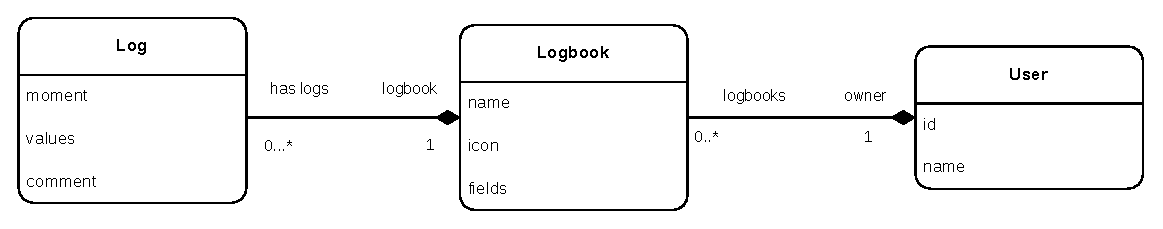
\includegraphics[width=0.8\textwidth]{conceptual-model.eps}
    \caption[Conceptual Model Diagram]{\label{fig:conceptmodel} Conceptual Model Diagram of the application}
\end{figure}

\begin{figure}[H]
    \centering
    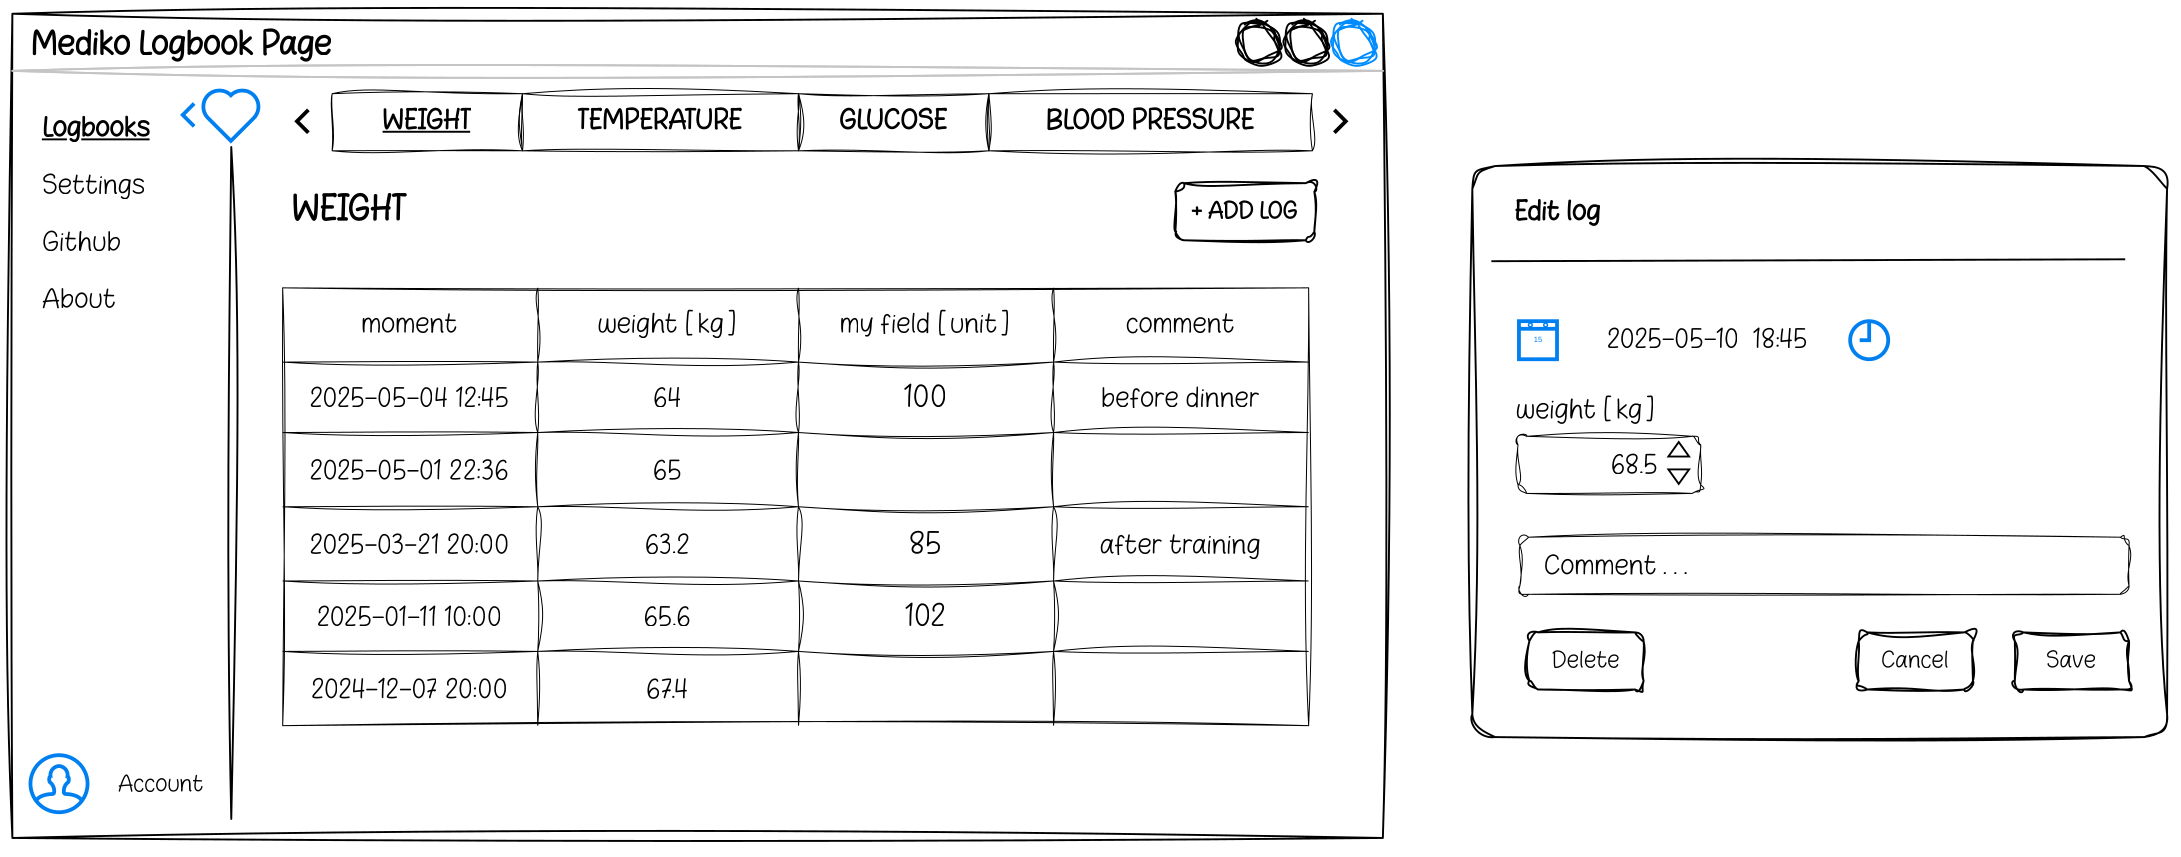
\includegraphics[width=0.8\textwidth]{layout-logbook.png}
    \caption[Logbooks page layout design]{\label{fig:layoutlogbook} Layout design of the logbooks page. Logbook Table (left), log edit menu (right) }
\end{figure}

On the Settings page user will be able to edit, remove and also create own custom logbooks with specified fields, units and (optionally) value precision. Before each line a checkbox will determine which logbooks should be visible on the tabs-bar on the Logbooks page. Before logbook deletion, an confirmation dialog must be shown.

\begin{figure}[H]
    \centering
    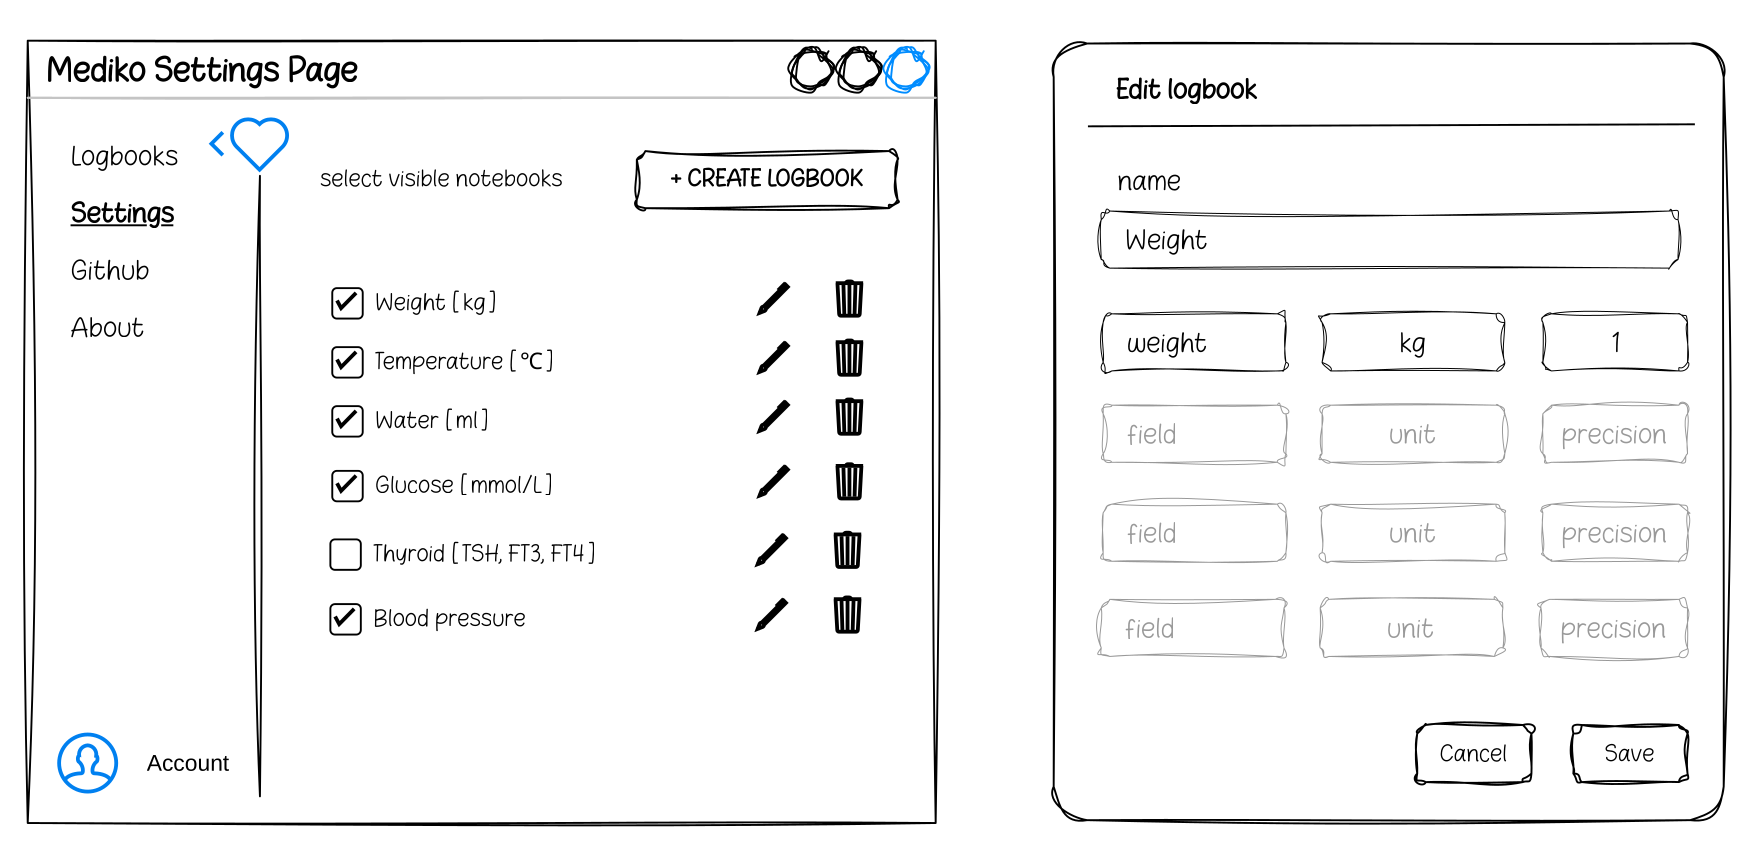
\includegraphics[width=0.8\textwidth]{layout-settings.png}
    \caption[Settings page layout design]{\label{fig:layoutsettings} Layout Design: Settings Page with available logbooks (left), logbook edit menu (right)}
\end{figure}

To achieve the greatest flexibility, client-server architecture will be used. One of the biggest advantages of this solution is the ability to share information resources among different users or devices belonging to the same user. In other words, data consistency is improved, what ensures all clients access the latest data from a one central source, minimizing divergences. Moreover centralized data storage allows for effective backups and management, enhancing data reliability. There is also possibility for errors isolation - client applications failures do not affect the server or other clients, what improves overall system stability making maintanace easier.
The intention is to allow the application to work completely in offline mode, and at the user's request or automatically in the background, synchronize the locally saved data with the cloud server. 

\begin{figure}[H]
    \centering
    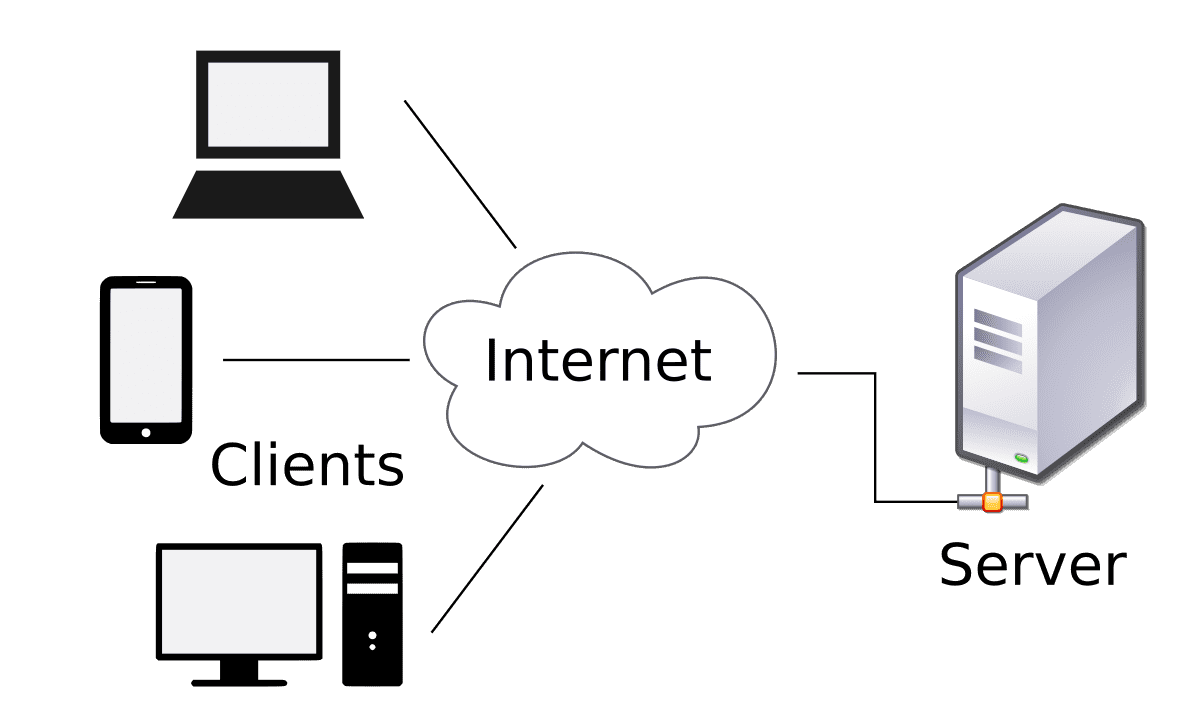
\includegraphics[width=0.8\textwidth]{client-server-architecture.png}
    \caption[Solution Architecture]{\label{fig:architecture} Solution client-server architecture }
\end{figure}

 

\section{{Language and framework choice}}

After a detailed analysis of the available solutions for writing the code, JavaScript was selected (or more precisely its extended variant - TypeScript). Below are the point arguments:

\begin{itemize}
  \item \textbf{Great popularity:} JavaScript seems to be the most widespread language across all devices types.
  \item \textbf{Wide range of available libraries and frameworks:} There are many popular JS libraries and frameworks available (mostly open-source) that can help implement desired functionalities.
  \item \textbf{Acceptable performance:} JavaScript uses so called Just-in-Time Compiler technique (JIT)\autocite{JIT}. At the runtime it's not the fastest language but unlike compiled languages (like for example C++) where the source code is converted into machine code before execution, it doesn't take much time to start up after making changes to the code because it doesn't need to go through that compilation step at the beginning.
\end{itemize}

To improve implementation of Object-Oriented Programming principles (OOP) both client and server will be written in TypeScript, a developed by Microsoft superset of JavaScript that adds optional static typing and other features to the language. TypeScript is compiled/transpiled into JavaScript, ensuring it works in all JS environments. Using TS can provide several advantages over plain JS, including:
\begin{itemize}
    \item \textbf{Static typing} allows programmers to define variable types and helps catch errors before running the code. It also improves quality and readability of the code.
    \item \textbf{Extra features} like generics, mapped types, utility-, intersection-, union- and conditional types, interfaces
    \item \textbf{Better Scalability:} TypeScript is used to manage and grow large projects. It makes it easier to maintain complex codebases over time.
\end{itemize}
\autocite{TSDoc} \autocite{TSfeatures}
\newline

Vue.js is one of the three most popular JavaScript framework (next to Angular, React) for building user  interfaces. It provides a declarative, component-based programming model that helps develop user interfaces of any complexity. According to the official documentation Vue.js has two most important core features:
\begin{itemize}
    \item \textbf{Declarative Rendering:} Vue extends standard HTML with a template syntax that allows developers to declaratively describe HTML output based on JavaScript state.
    \item \textbf{Reactivity:} Vue automatically tracks JavaScript state changes and efficiently updates the DOM when changes happen.
\end{itemize}


Programmers can choose between two coding styles:
\begin{itemize}
    \item \textbf{Options API} is the traditional method of building Vue components and has been a core feature of Vue since its inception. The Options API in Vue organizes component logic into clearly defined options like data, methods, and computed, offering a familiar and structured approach to managing component behavior.
    \item \textbf{Composition API} is a newer way of building components in Vue since version 3 that was introduced to address some of the limitations of the Options API. The Composition API in Vue allows developers to use a functional, reactive programming style to build components, and it offers a more flexible and expressive way of defining component behavior.
\end{itemize}
Each approach brings its own set of advantages and challenges, making the decision on which one to use a critical consideration for any project. In this thesis for the proof-of-concept project the newer Composition API will be used.

\begin{listing}[H]
    \begin{minted}{vue}
    <template>
        <div>
            <p>{{ props.title }}</p>
            <p @click="increment">Clicks: {{ clickCount }}</p>
        </div>
    </template>
    
    <script setup lang="ts">
    import { Ref, ref } from "vue";
    interface ExampleProps {
        title: string;
    }
    const props = defineProps<ExampleProps>();
    const clickCount: Ref<number> = ref(0);
    function increment() {
        clickCount.value += 1;
        return clickCount.value;
    }
    </script>
    
    <style lang="css">
    p {
        color: red;
    }
    </style>
    \end{minted}
\caption[Vue document example]{Example of .vue document including 3 sections: \newline <template> : where html document structure is defined, \newline<script> : with example TypeScript code, \newline<style> : containing CSS style for current component}
\end{listing}

Quasar is an an MIT licensed open-source js framework build on top of the Vue.js using its reactivity and component-based architecture. It offers a wide range of customizable pre-built UI components (such as buttons, forms, tables, infinite scrolling, dialogs, notifications, etc...) allowing developers to focus on implementing functionalities. Quasar has built-in support for responsive and mobile-first design. Its biggest benefit is the availability of all features in one place, accessible from the CLI level and online documentation.
Through the CLI built-in functions framework allows to test and deploy once written code simultaneously as a website, a Mobile App and/or an standalone Desktop Application. \autocite{QuasarStart}

\section{\IfLanguageName{dutch}{Voorbereiding}{Prerequisites}}%
\label{sec:prerequisites}

The software is being developed on a PC machine with x64 architecture running Fedora Linux. The project  will be managed on the Azure DevOps where tasks are described and issues tracked. GitHub repository was initialized for code version control and cloned locally. The machine has already installed Node.js - a JavaScript runtime environment, Node Package Manager (npm) and Node Version Manager (nvm). Detailed installation is not a subject of this thesis.

Quasar framework provides own command line interface (CLI) allowing access to more features and automating some tasks. The CLI will be installed globally to make possible to directly run Quasar commands in the terminal, run a local http server for testing or do upgrades on the project \autocite{QuasarStart}. According to the Quasar documentation, the following code needs to be executed:

\begin{verbatim}
    npm i -g @quasar/cli

\end{verbatim}

\section{\IfLanguageName{dutch}{Installatie}{Client Template Installation}}%
\label{sec:installation}

New Quasar project is initialised with the command:
\begin{verbatim}
    npm init quasar@latest

\end{verbatim}

Installation wizard asks some questions about preferences to automatically generate startup project template. The developer chooses first a project type (in most cases it's an application) and folder name. Command is executed inside already initialised git repo, so folder 'client' becomes a subfolder of the whole project repository. 

\begin{verbatim}
? What would you like to build? > - Use arrow-keys. Return to submit.
>  App with Quasar CLI, let's go! - spa/pwa/ssr/bex/electron/capacitor/cordova
   AppExtension (AE) for Quasar CLI
   Quasar UI kit
   
? Project folder: > client

\end{verbatim}

The next question is about choosing the project language. For better support of the OOP paradigm, it is recommended to choose TypeScript, which extends JavaScript, among others, the possibility of type declaration \autocite{TSDoc}
\begin{verbatim}
    ? Pick script type: >
        Javascript
    >   Typescript

\end{verbatim}

The default and recommended by Vue.js and Quasar local UI development server is Vite including a Hot Module Replacement (HMR) system, which works by just reloading the specific file being changed instead of recompiling the entire application \autocite{Vite}. 
\begin{verbatim}
    ? Pick Quasar App CLI variant: >
    >   Quasar App CLI with Vite - recommended
        Quasar App CLI with Webpack

\end{verbatim}    

Vue.js comes with two programmings styles, the newer one - Composition API is recommended because of better TypeScript support \autocite{VueAPIStyles}
% add reference to detailed description
\begin{verbatim}
    ? Pick a Vue component style: > 
    >   Composition API with <script setup> - recommended
        Composition API
        Options API

\end{verbatim}

\begin{verbatim}
    ? Pick your CSS preprocessor: > 
    >   Sass with SCSS syntax
        Sass with indented syntax
        None (the others will still be available)
\end{verbatim}

Additional package(s) suggested by the CLI, in this case Pinia State Management and Axios (promise based HTTP client for the web-browser and node.js) are choosen.
% add reference to detailed description
\begin{verbatim}
    ? Check the features needed for your project: >  
    ◯   Linting (vite-plugin-checker + ESLint + vue-tsc)
    ◉   State Management (Pinia)
    ◉   axios
    ◯   vue-i18n
    
    Quasar •  SUCCESS  • The project has been scaffolded

    ? Install project dependencies? (recommended)
    >   Yes, use npm
        No, I will handle that myself 

\end{verbatim}
    

Quasar CLI shows the summary of choosen options:

\begin{verbatim}
What would you like to build? > App with Quasar CLI, let's go!
Project folder: … client
Pick script type: > Typescript
Pick Quasar App CLI variant: > Quasar App CLI with Vite
Package name: … mediko-client
Project product name: > … Mediko
Project description: > … Cross-platform application with Vue, Quasar
Pick a Vue component style: > Composition API with <script setup>
Pick your CSS preprocessor: > Sass with SCSS syntax
Check the features needed for your project: > State Management (Pinia), axios
\end{verbatim}

\section{\IfLanguageName{dutch}{Web client applicatie}{Single Page Application Web Client}}%
\label{sec:webclient}

To start the web application in browser with Quasar CLI we need to navigate to the client folder and call Quasar CLI dev command.

\begin{verbatim}
    cd client
    quasar dev
\end{verbatim}

The template is now working - project startup applications automatically opens in default browser:

\begin{figure} [H]
    \centering
    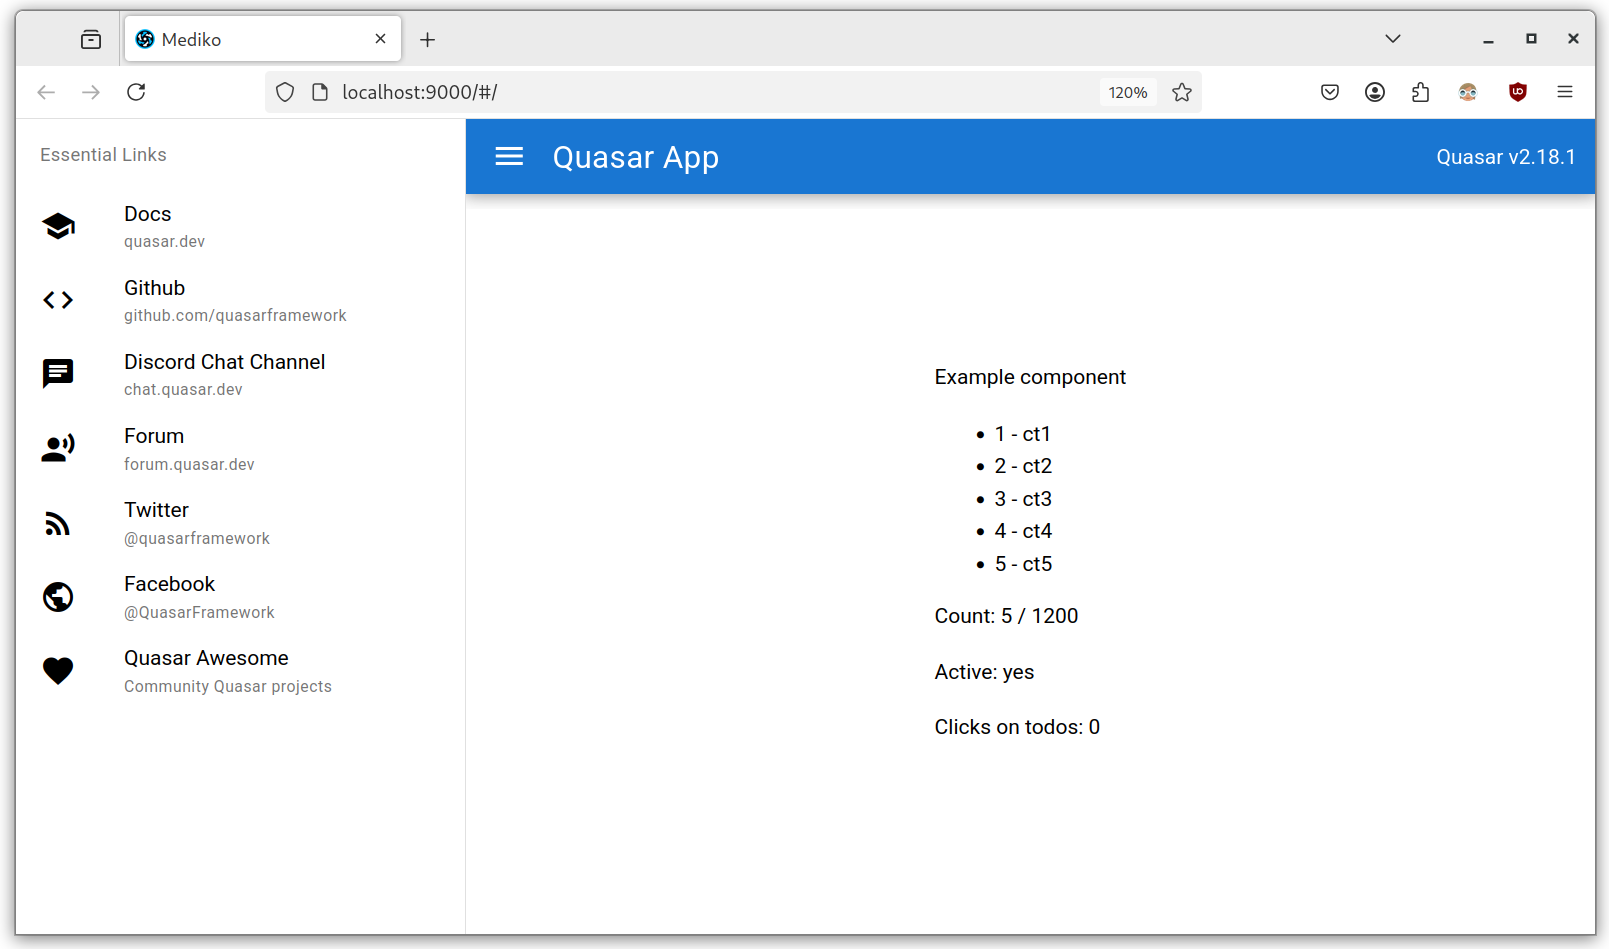
\includegraphics[width=0.8\textwidth]{templ-layout.png}
    \caption[Client Template]{\label{fig:template}Created Project template in the web browser.}
\end{figure}

Initially, the project contains an example clicks-counter and some Quasar related navigation links in the drawer, they will be removed in the next step to prepare template for implementations of proof-of-concept functionalities.


\section{{Implementation of Functionalities}}%
\label{sec:functionalities}
% Logbooks, log, edit logs, 
% class diagram
% Local Storage

In the first step, entity models were created in apart folder (Logbook and Log). They both inherit properties from abstract class TrackedEntity, which contains identity property as uuid (128-bit values that are canonically represented as a 36-character string in the format 123e4567-e89b-12d3-a456-426614174000, 5 hex strings separated by hyphens) string \autocite{UUID}, it allows multiple clients independently create items without conflict during synchronization.

\begin{listing}[H]
    \begin{minted}{ts}
    import { v4 as uuidv4 } from 'uuid';
    export class TrackedEntity {
        id: string = uuidv4();
        createdAt?: Date;
        updatedAt?: Date;
        deletedAt?: Date | null = null;
        isDeleted?: boolean = false;
    }
    \end{minted}
\caption[Tracked Entity]{Abstract TrackedEntity inherited by Mediko Entity classes Log, Logbook}
\end{listing}


The client application design model is described by the diagram below:

\begin{figure}[H]
    \centering
    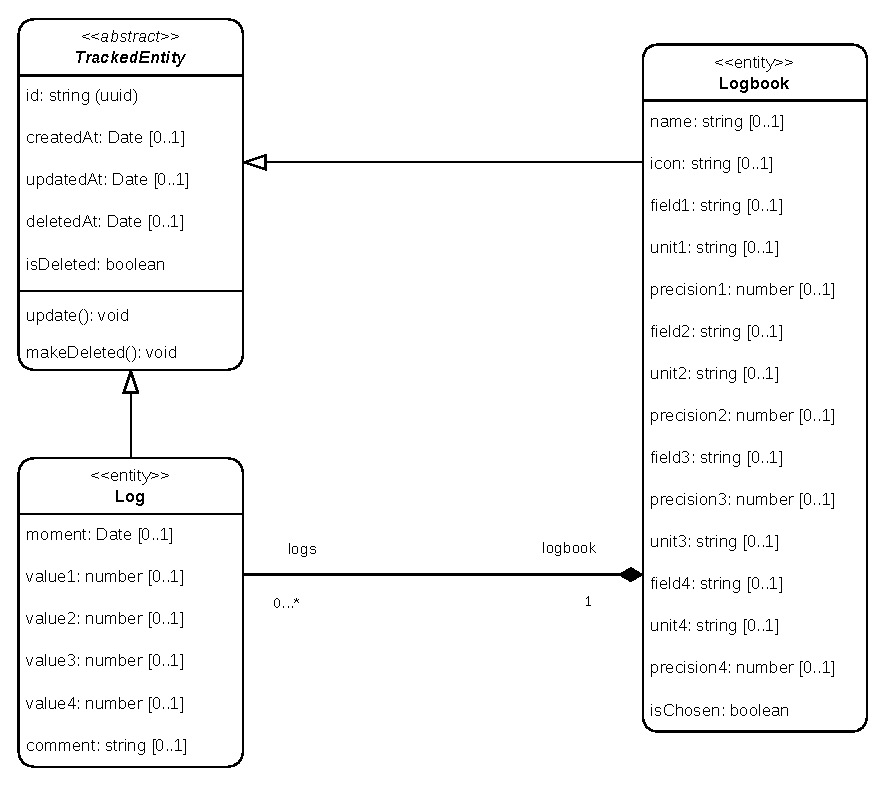
\includegraphics[width=0.8\textwidth]{info-design-model.eps}
    \caption[Class Diagram]{\label{fig:infomodeldiagram} Client App Information Design Model Class Diagram }
\end{figure}

Data management methods are seperated from the model view logic and placed in apart service class  (LogbookLocalService). Mediko has to work independently as standalone application, so data are saved in browser LocalStorage and preserved as long as the browser cache will not be cleared. Quasar framework provides already included wrapper around Web Storage API - mechanisms by which browsers can store key/value pairs \autocite{MozillaLocalStorage}.

\begin{figure}[H]
    \centering
    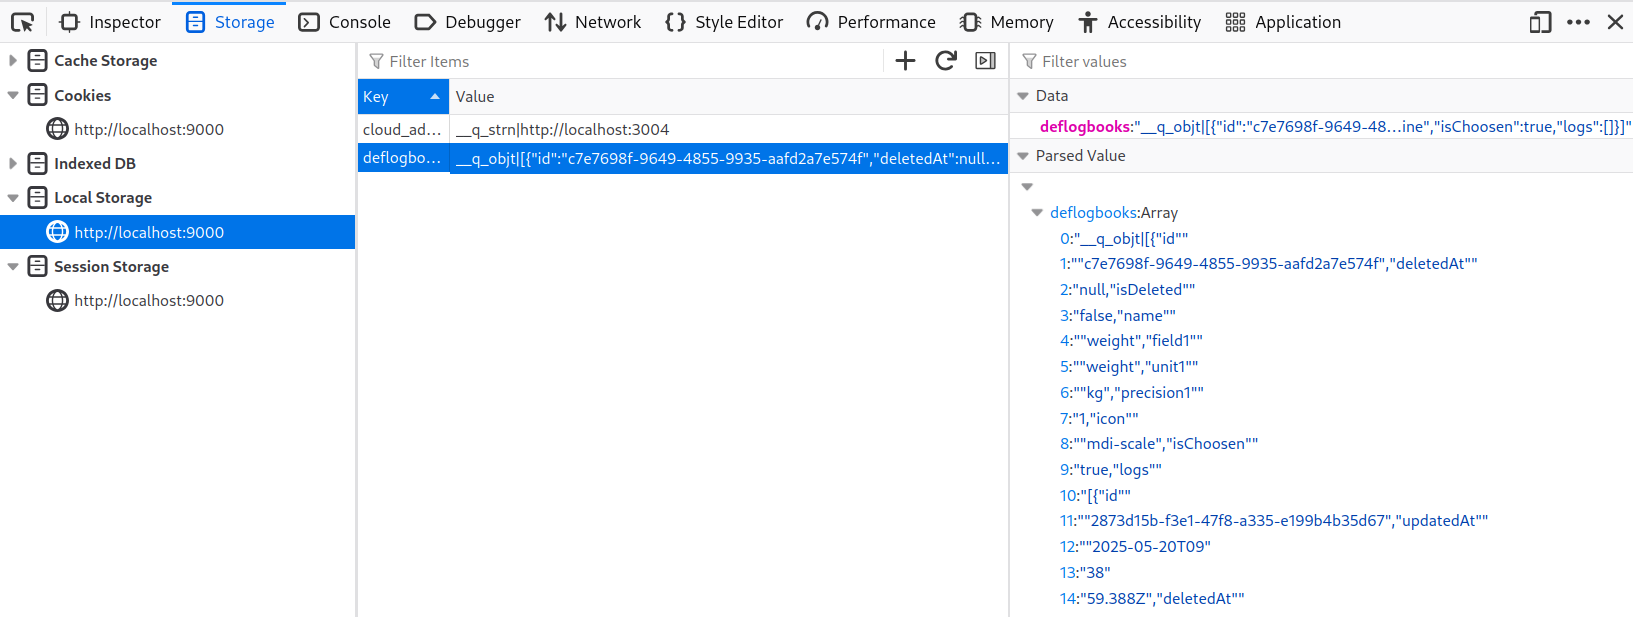
\includegraphics[width=0.8\textwidth]{local-storage.png}
    \caption[LocalStorage]{\label{fig:localstorage} Local Storage in Firefox Dev Tools }
\end{figure}

\begin{figure}[H]
    \centering
    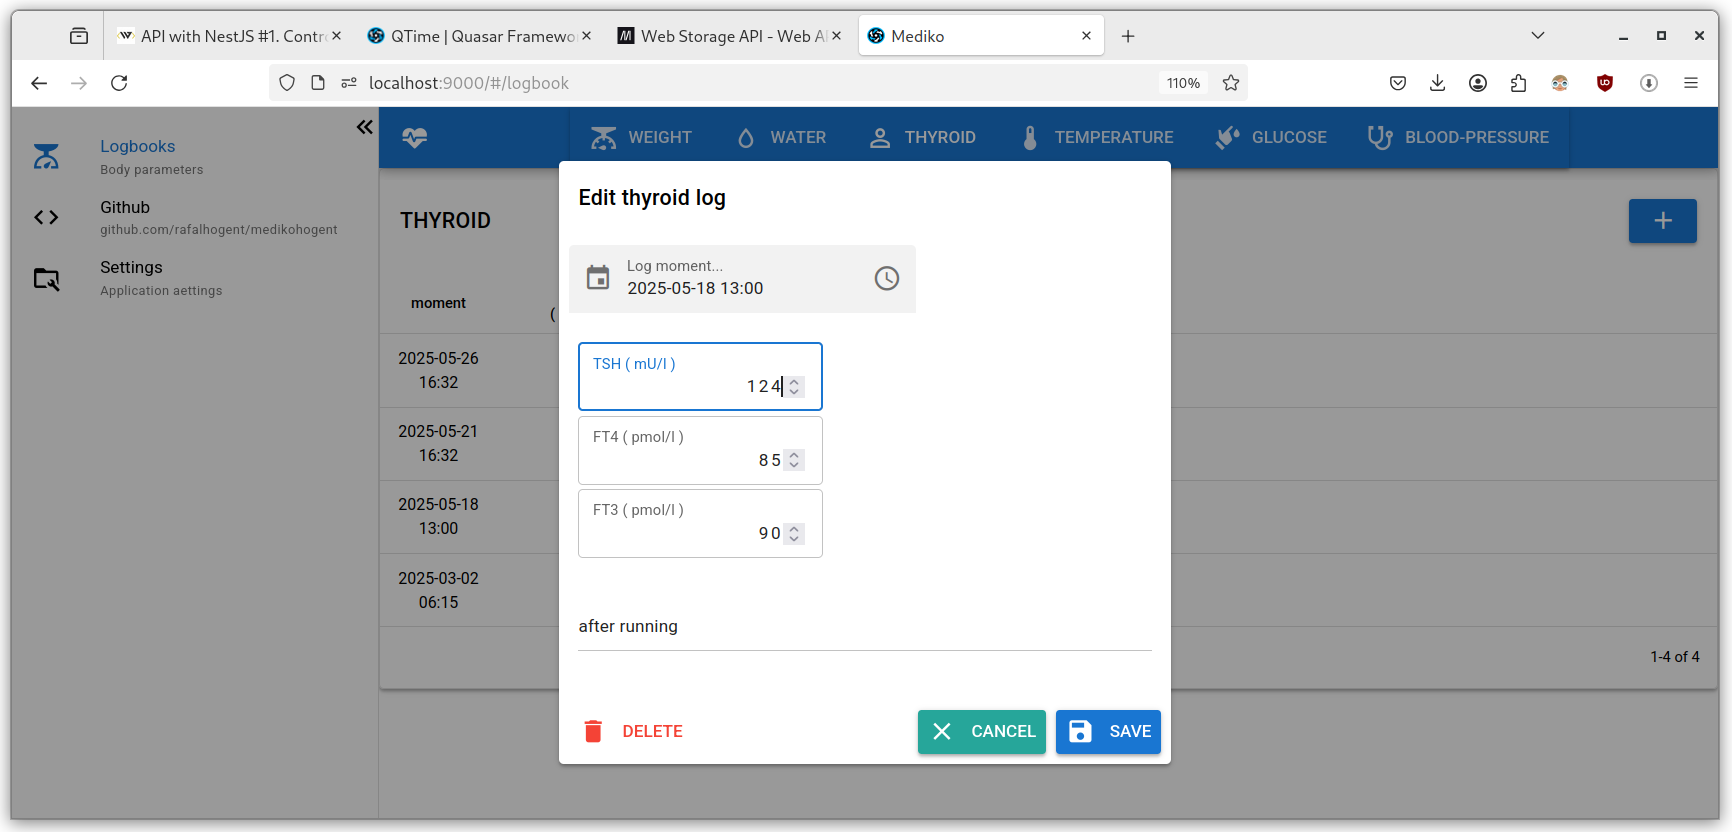
\includegraphics[width=0.7\textwidth]{screen-editlog.png}
    \caption[Editing Log in Web Browser]{\label{fig:editlogs} Mediko web application running in web browser. Editing logs menu }
\end{figure}


\begin{figure}[H]
    \centering
    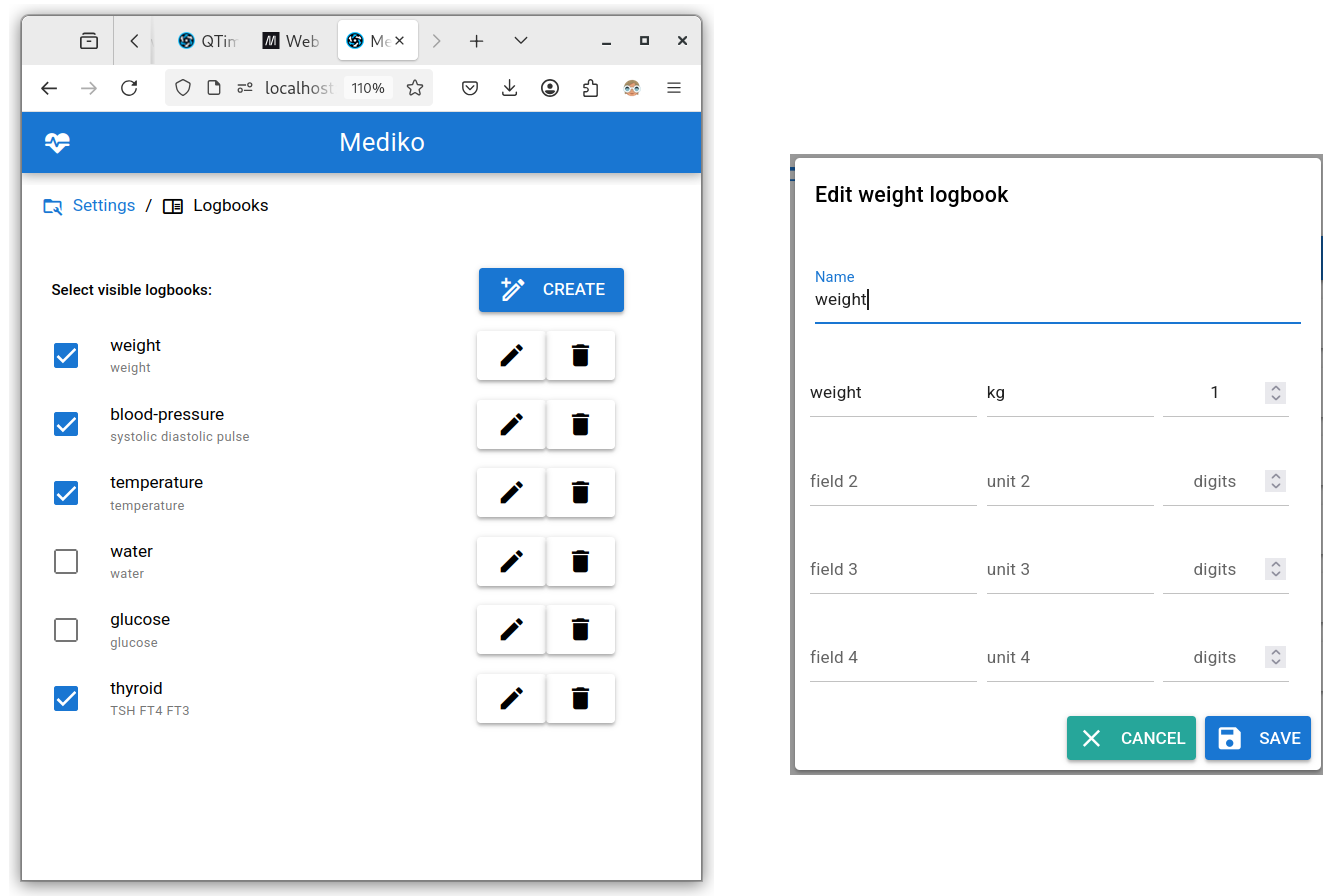
\includegraphics[width=0.7\textwidth]{screen-settings.png}
    \caption[Screen settings]{\label{fig:settings} Screen settings and editing logbooks. }
\end{figure}

    

\begin{listing}[H]
    \begin{minted}{ts}
import { LocalStorage } from "quasar";
export class LogbookLocalService {
  static getLocalLogbooks(): Logbook[] {
    const localLogbooks = plainToInstance(
      Logbook,
      LocalStorage.getItem(DEF_LOGBOOKS) as any[]
    );
    if (Array.isArray(localLogbooks) && localLogbooks?.length) {
      const deflogbooks = localLogbooks?.filter((lb) => !lb.isDeleted);
      deflogbooks.forEach((lgb) => {
        lgb.logs = lgb.logs
          .filter((l) => !l.isDeleted)
          .map((l) => plainToInstance(Log, l));
        lgb.logs.forEach((l) => {
          if (l.moment) {
            l.moment = DateTime.fromISO(l.moment.toString()).toJSDate();
          }
        });
      });
      return deflogbooks;
    }
    return [];
  }

  static saveLogbooksData(logbooks: Logbook[]) {
    LocalStorage.setItem(DEF_LOGBOOKS, logbooks);
  }
}
    \end{minted}
\caption[Logbook Local Service]{Client local data storage implementation, part of the featured LogbookLocalService class}
\end{listing}



In the application repository client folder is organized in structured subfolders. In the 'pages 'folder are located vue files representing pages-components used by vue-router \autocite{VueRouter}. Folder 'models' contains entities and view-models definition in typescript. Folder 'services' contains 'local' subfolder where are located classes responsible for data management in client local storage, later will be added subfolder with classes responsible for external communication (like data synchronization). The full source code is available on the Github repository attached to the thesis.

\begin{listing}[H]
    \begin{minted}{shell}
        client
        ├── src
            ├── App.vue
            ├── assets
            ├── boot
            ├── components
            │   ├── common
            │   │   └── Confirmation.vue
            │   ├── EssentialLink.vue
            │   └── logbook
            │       ├── EditLogbook.vue
            │       └── EditLog.vue
            ├── css
            ├── layouts
            │   └── MainLayout.vue
            ├── models
            │   ├── common
            │   │   └── tracked-entity.ts
            │   └── logbook
            │       ├── logbook.ts
            │       └── log.ts
            ├── pages
            │   ├── ErrorNotFound.vue
            │   ├── IndexPage.vue
            │   ├── LogbookPage.vue
            │   ├── settings-pages
            │   │   ├── LogbooksSettingsPage.vue
            │   │   └── MainSettingsPage.vue
            │   └── SettingsPage.vue
            ├── router
            │   ├── index.ts
            │   └── routes.ts
            ├── services
            │   └── local
            │       ├── local-keys.ts
            │       └── logbook.local.service.ts
            └── stores
                ├── app.store.ts
                └── index.ts
    \end{minted}
\caption[]{Client Repository folder structure tree}
\end{listing}


% Voeg hier je eigen hoofdstukken toe die de ``corpus'' van je graduaatsproef
% vormen. De structuur en titels hangen af van je eigen onderzoek. Je kan bv.
% elke fase in je onderzoek in een apart hoofdstuk bespreken.

%\input{...}
%\input{...}
%...

%%=============================================================================
%% Conclusie
%%=============================================================================

\chapter{\IfLanguageName{dutch}{Conclusie}{Conclusion}}%
\label{ch:conclusie}

TODO: Trek een duidelijke conclusie, in de vorm van een antwoord op de
onderzoeksvra(a)g(en). Wat was jouw bijdrage aan het onderzoeksdomein en
hoe biedt dit meerwaarde aan het vakgebied/doelgroep? 
Reflecteer kritisch over het resultaat. In Engelse teksten wordt deze sectie
'Discussion' genoemd. Had je deze uitkomst verwacht? Zijn er zaken die nog
niet duidelijk zijn?
Heeft het onderzoek geleid tot nieuwe vragen die uitnodigen tot verder 
onderzoek?



%---------- Bijlagen -----------------------------------------------------------

\appendix

\chapter{Onderzoeksvoorstel}

Het onderwerp van deze graduaatsproef is gebaseerd op een onderzoeksvoorstel dat vooraf werd beoordeeld door de promotor. Dat voorstel is opgenomen in deze bijlage.

%% TODO: 
\section*{Samenvatting}

% Kopieer en plak hier de samenvatting (abstract) van je onderzoeksvoorstel.
  %  Hier schrijf je de samenvatting van je voorstel, als een doorlopende tekst van één paragraaf. Let op: dit is geen inleiding, maar een samenvattende tekst van heel je voorstel met inleiding (voorstelling, kaderen thema), probleemstelling en centrale onderzoeksvraag, onderzoeksdoelstelling (wat zie je als het concrete resultaat van je bachelorproef?), voorgestelde methodologie, verwachte resultaten en meerwaarde van dit onderzoek (wat heeft de doelgroep aan het resultaat?).
  De graduaatsproef zal proberen antwoord te geven op de vraag of de softwareontwikkelingsmethode op basis van het gebruik van één broncode in JavaScript en TypeScript \autocite{TSDoc} en publicatie op vele platformen effectief betrouwbaar werkende applicatie kan leveren. Die methode kan zeer nuttig zijn voor programmeurs die hun code als standalone applicatie ook kunnen publiceren. Er zal gebruik gemaakt worden van technologieën zoals: Quasar \autocite{QuasarStart}, Vue \autocite{VueDoc}, NestJs \autocite{NestJsDoc}, Electron \autocite{ElectronDoc} en Cordova \autocite{CordovaDoc}.

% Verwijzing naar het bestand met de inhoud van het onderzoeksvoorstel
%---------- Inleiding ---------------------------------------------------------

% TODO: Is dit voorstel gebaseerd op een paper van Research Methods die je
% vorig jaar hebt ingediend? Heb je daarbij eventueel samengewerkt met een
% andere student?
% Zo ja, haal dan de tekst hieronder uit commentaar en pas aan.

%\paragraph{Opmerking}

% Dit voorstel is gebaseerd op het onderzoeksvoorstel dat werd geschreven in het
% kader van het vak Research Methods dat ik (vorig/dit) academiejaar heb
% uitgewerkt (met medesturent VOORNAAM NAAM als mede-auteur).
% 

\section{Inleiding}%
\label{sec:inleiding}

Mijn graduaatsproef zal gaan over de ontwikkeling van een cross-platform applicatie met gebruik maken van TypeScript/JavaScript \autocite{TSDoc}. Het wordt een applicatie die gebruikers laat hun gegevens (bv. medische metingen) noteren, bewaren en synchroniseren met de server, waardoor andere clients er toegang toe krijgen. Ik wil dat mijn applicatie volledig offline kan werken, de gegevens zullen in de Local Storage \autocite{MozillaLocalStorage} bewaard en op aanvraag gesynchroniseerd.

Mijn werk kan nuttig zijn voor alle ontwikkelaars die zich hebben beperkt tot het publiceren van hun producten alleen als webapplicaties, terwijl standalone applicaties handiger kunnen zijn voor gebruikers. Vanwege de geplande functionaliteiten van mijn applicatie kunnen ziekenhuizen of wijkgezondheidscentra overwegen om deze te implementeren om op afstand door patiënten zelf ingevulde gegevens te kunnen verzamelen.

Mijn onderzoeksvraag:
\textbf{Welke voordelen en moeilijkheden kunnen we krijgen bij het maken van applicaties voor meerdere platformen met gebruik maken van één enkele codebron in JS/TS, het Quasar-framework, Electron en Cordova? }

%---------- Stand van zaken ---------------------------------------------------

\section{Literatuurstudie}%
\label{sec:literatuurstudie}

In het geval van applicatieontwikkeling zal het gebruik van literatuur vooral plaatsvinden in de online documentatie van de gebruikte frameworks en op web-pagina's zoals StackOverflow \autocite{StackOverflow} en Github \autocite{Github} op zoek naar oorzaken en oplossingen voor technische problemen.

% Voor literatuurverwijzingen zijn er twee belangrijke commando's:
% \autocite{KEY} => (Auteur, jaartal) Gebruik dit als de naam van de auteur
%   geen onderdeel is van de zin.
% \textcite{KEY} => Auteur (jaartal)  Gebruik dit als de auteursnaam wel een
%   functie heeft in de zin (bv. ``Uit onderzoek door Doll & Hill (1954) bleek
%   ...'')

% Je mag deze sectie nog verder onderverdelen in subsecties als dit de structuur van de tekst kan verduidelijken.

%---------- Methodologie ------------------------------------------------------
\section{Methodologie}%
\label{sec:methodologie}

Het onderzoek zal uitgevoerd worden door het maken van PoC (proef of concept) applicatie en het lezen van de online documentatie van bepaalde frameworks.
Graduaatsproef als applicatieontwikkeling is een taak die niet alleen kennis van programmeertalen vereist, maar ook technische vaardigheden, dus het kan alleen worden gemaakt door mensen met IT-achtergrond.
Het project zal gemaakt worden op een PC laptop met Linux en Windows als virtuele machine (VirtualBox) \autocite{VBox}. De code wordt geschreven in de Visual Studio Code \autocite{Vscode}, samen met extensies die zijn gewijd aan TypeScript en Vue \autocite{VueDoc}. Ik ga ook gebruik maken van Android emulator \autocite{AndroidDev} om mobile versie van de applicatie te kunnen testen.\newline


Ik voorzie onderstaande fases van het werk:
\begin{itemize}
  \item Onderzoek van beschikbare cross-platform oplossingen
  \item Een werkende PoC-template applicatie leveren voor alle platformen (Web, Desktop (Windows en Linux), Mobile (Android)) 
  \item Layout design, Domein- en architectuuranalyse met respect voor OOP \autocite{NyakundiOOP}
  \item Implementatie van de functionaliteiten
  \item Frontend applicatie koppelen met backend in NestJs \autocite{NestJsDoc}
\end{itemize}

Mijn Graduaatsproef zal in het Engels geschreven worden.


%---------- Verwachte resultaten ----------------------------------------------
\section{Verwacht resultaat, conclusie}%
\label{sec:verwachte_resultaten}

% Hier beschrijf je wat je verwacht uit je onderzoek, met de motivatie waarom. Het is \textbf{niet} erg indien uit je onderzoek andere resultaten en conclusies vloeien dan dat je hier beschrijft: het is dan juist interessant om te onderzoeken waarom jouw hypothesen niet overeenkomen met de resultaten.

Als resultaat verwacht ik een stabiel werkende applicatie die identiek eruitziet op alle platformen. De ontwikkeling proces moet ook snel en effectief zijn, met andere woorden wil ik graag nagaan welke moeilijkheden zich tijdens het ontwikkelingsproces kunnen voordoen, waardoor het werk kan worden vertraagd of de kwaliteit kan worden verlaagd. Elk software-ontwikkelingsbedrijf kan veel tijd en dus geld besparen als het product voor alle platforms kan worden getest en gepubliceerd met behulp van één enkele codebron.





%%---------- Andere bijlagen --------------------------------------------------
% TODO: Voeg hier eventuele andere bijlagen toe. Bv. als je deze BP voor de
% tweede keer indient, een overzicht van de verbeteringen t.o.v. het origineel.
%\input{...}

%%---------- Backmatter, referentielijst ---------------------------------------

\backmatter{}

\setlength\bibitemsep{2pt} %% Add Some space between the bibliograpy entries
\printbibliography[heading=bibintoc]

\end{document}
